\documentclass[10pt,a4paper]{article}
\usepackage[utf8]{inputenc}

% Define the page margin
\usepackage[margin=3cm]{geometry}

% Better typography (font rendering)
\usepackage{microtype}

% Math environments and macros
\usepackage{amsmath}
\usepackage{amsfonts}
\usepackage{amssymb}
\usepackage{amsthm}

% Define \includegraphics to include graphics
\usepackage{graphicx}

% Draw graphics from a text description
\usepackage{tikz}

% Syntax highlighting
\usepackage{minted}

% Set global minted options
\setminted{linenos, autogobble, frame=lines, framesep=2mm}

% Import the comment environment for orgtbl-mode
\usepackage{comment}

% Do not indent paragraphs
\usepackage{parskip}

\title{Operating Systems, Sheet 7}
\author{Marten Lienen (03670270)}

\begin{document}

\maketitle

\section*{Exercise 1}

\subsection*{Part 1.1)}

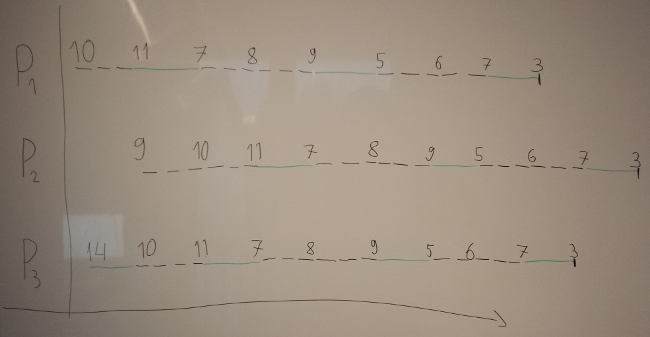
\includegraphics[width=\textwidth]{sheet-7/exercise-1-1}

\subsection*{Part 1.2)}

% BEGIN RECEIVE ORGTBL exercise-1-2
\begin{tabular}{rrrrrr}
$i$ & $a_{i}$ & $b_{i}$ & $c_{i}$ & $v_{i}$ & $w_{i}$\\
\hline
1 & 0 & 6 & 16 & 16 & 10\\
2 & 2 & 6 & 20 & 18 & 12\\
3 & 0 & 8 & 18 & 18 & 10\\
\end{tabular}
% END RECEIVE ORGTBL exercise-1-2
\begin{comment}
#+ORGTBL: SEND exercise-1-2 orgtbl-to-latex :splice nil :skip 0 :raw t
| $i$ | $a_{i}$ | $b_{i}$ | $c_{i}$ | $v_{i}$ | $w_{i}$ |
|-----+---------+---------+---------+---------+---------|
|   1 |       0 |       6 |      16 |      16 |      10 |
|   2 |       2 |       6 |      20 |      18 |      12 |
|   3 |       0 |       8 |      18 |      18 |      10 |
\end{comment}

\begin{equation*}
  \bar{V} = \frac{16 + 18 + 18}{3} = \frac{52}{3} \approx 17.3 \qquad \bar{W} = \frac{10 + 12 + 10}{3} = \frac{32}{3} \approx 10.7
\end{equation*}

\section*{Exercise 2}

\subsection*{Part 2.1)}

\subsection*{Part 2.2)}

\begin{itemize}
\item Der PCB ist eine Datenstruktur, die alle Attribute enthält, die einen Prozess beschreiben (z.B. PID und Priorität)
\item Beim Scheduling braucht man den PCB um die aktuelle Priorität und Position in der Warteschlange zu speichern.
  Für das Dispatching sind z.B. die gespeicherten Registerwerte wichtig, die wiederhergestellt werden müssen.
\item Die aktuelle Belegung der Prozessoren und wohin der ausgewählte Prozess geschickt werden soll
\item Bei Threads müssen können viele Werte und Einstellungen (z.B. gemappte Memory-Pages) gleich bleiben.
  Bei Prozessen müssen diese ausgetauscht werden.
  Wenn die Threads nur auf User-Level implementiert sind, hat der Dispatcher damit gar nichts zu tun.
\item Der Dispatcher lädt und stoppt die Prozesse, die der Scheduler ausgewählt hat.
\item Zuerst speichert man die Registerinhalte.
  Dann vielleicht noch die aktuell geladenen Memory-Pages.
\item Je größer die PCBs sind, desto mehr Arbeit muss der Dispatcher bei jedem Kontextwechsel verrichten.
  Ein großer PCB verringert also die Effizienz des Gesamtsystems.
\end{itemize}

\subsection*{Part 2.3)}

\subsubsection*{First-Come-First-Served}

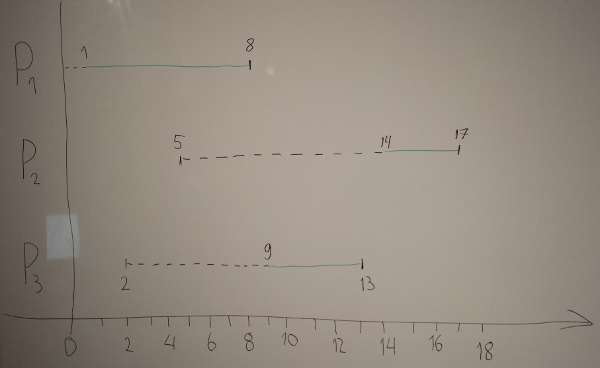
\includegraphics[width=\textwidth]{sheet-7/exercise-2-3-1}

\begin{equation*}
  \bar{V} = \frac{8 + 12 + 11}{3} = \frac{31}{3} \approx 10.3 \qquad \bar{W} = \frac{1 + 7 + 9}{3} = \frac{17}{3} \approx 5.7
\end{equation*}

\subsubsection*{Shortest-Remaining-Processing-Time}

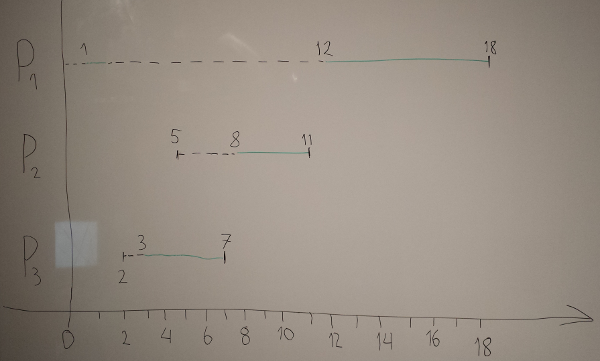
\includegraphics[width=\textwidth]{sheet-7/exercise-2-3-2}

\begin{equation*}
  \bar{V} = \frac{18 + 6 + 5}{3} = \frac{29}{3} \approx 9.7 \qquad \bar{W} = \frac{1 + 3 + 11}{3} = 5
\end{equation*}

\subsubsection*{Round-Robin Scheibenlänge 1}

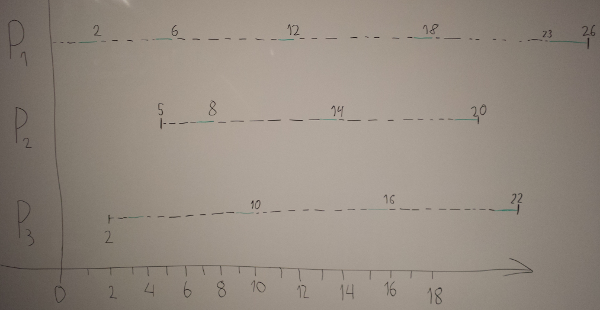
\includegraphics[width=\textwidth]{sheet-7/exercise-2-3-3}

\begin{equation*}
  \bar{V} = \frac{26 + 15 + 20}{3} = \frac{61}{3} \approx 20.3 \qquad \bar{W} = \frac{19 + 12 + 16}{3} = \frac{47}{3} \approx 15.7
\end{equation*}

\subsubsection*{Round-Robin Scheibenlänge 2}

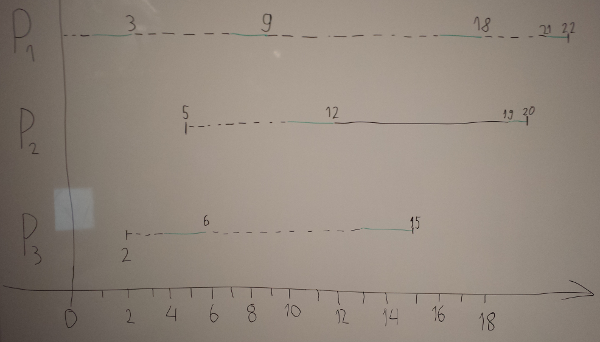
\includegraphics[width=\textwidth]{sheet-7/exercise-2-3-4}

\begin{equation*}
  \bar{V} = \frac{22 + 15 + 13}{3} = \frac{50}{3} \approx 16.7 \qquad \bar{W} = \frac{15 + 12 + 9}{3} = 12
\end{equation*}

\subsubsection*{Fragen}

Die kürzeste Wartzeit tritt bei Shortest-Remaining-Processing-Time auf.

Längere Zeitquanten erhöhen die Effizienz auf Kosten einer potentiell längeren Wartezeit bis zur ersten Rechnung nachdem ein Prozess in der Schedulingwarteschlange ankommt.

\section*{Exercise 3}

\subsection*{Part 3.1)}

% BEGIN RECEIVE ORGTBL short-term-scheduling
\begin{tabular}{lrrrrrrrrrrr}
Zeit & 0 & 1 & 2 & 3 & 4 & Recompute & 5 & 6 & 7 & 8 & Recompute\\
\hline
Zeit 1 & 10 &  & 9 &  &  & 9 & 8 &  & 7 & 6 & 6\\
Prio 1 & 3 &  & 3 &  &  & 5 & 5 &  & 5 & 5 & 8\\
p\_cpu 1 & 0 &  & 8 &  &  & 6 & 14 &  & 22 & 30 & 20\\
Zeit 2 & 1 &  &  & 0 &  &  &  &  &  &  & \\
Prio 2 & 1 &  &  & 1 &  &  &  &  &  &  & \\
p\_cpu 2 & 0 &  &  & 8 &  &  &  &  &  &  & \\
Zeit 3 & 2 &  &  &  & 1 & 1 &  & 0 &  &  & \\
Prio 3 & 3 &  &  &  & 3 & 5 &  & 5 &  &  & \\
p\_cpu 3 & 0 &  &  &  & 8 & 6 &  & 14 &  &  & \\
Zeit 4 & 1 & 0 &  &  &  &  &  &  &  &  & \\
Prio 4 & 4 & 4 &  &  &  &  &  &  &  &  & \\
p\_cpu 4 & 0 & 8 &  &  &  &  &  &  &  &  & \\
Zeit 5 & 5 &  &  &  &  & 5 &  &  &  &  & 5\\
Prio 5 & 2 &  &  &  &  & 2 &  &  &  &  & 2\\
p\_cpu 5 & 0 &  &  &  &  & 0 &  &  &  &  & 0\\
\end{tabular}
% END RECEIVE ORGTBL short-term-scheduling
\begin{comment}
#+ORGTBL: SEND short-term-scheduling orgtbl-to-latex :splice nil :skip 0 :raw t
| Zeit     |  0 | 1 | 2 | 3 | 4 | Recompute |  5 |  6 |  7 |  8 | Recompute |
|----------+----+---+---+---+---+-----------+----+----+----+----+-----------|
| Zeit 1   | 10 |   | 9 |   |   |         9 |  8 |    |  7 |  6 |         6 |
| Prio 1   |  3 |   | 3 |   |   |         5 |  5 |    |  5 |  5 |         8 |
| p\_cpu 1 |  0 |   | 8 |   |   |         6 | 14 |    | 22 | 30 |        20 |
| Zeit 2   |  1 |   |   | 0 |   |           |    |    |    |    |           |
| Prio 2   |  1 |   |   | 1 |   |           |    |    |    |    |           |
| p\_cpu 2 |  0 |   |   | 8 |   |           |    |    |    |    |           |
| Zeit 3   |  2 |   |   |   | 1 |         1 |    |  0 |    |    |           |
| Prio 3   |  3 |   |   |   | 3 |         5 |    |  5 |    |    |           |
| p\_cpu 3 |  0 |   |   |   | 8 |         6 |    | 14 |    |    |           |
| Zeit 4   |  1 | 0 |   |   |   |           |    |    |    |    |           |
| Prio 4   |  4 | 4 |   |   |   |           |    |    |    |    |           |
| p\_cpu 4 |  0 | 8 |   |   |   |           |    |    |    |    |           |
| Zeit 5   |  5 |   |   |   |   |         5 |    |    |    |    |         5 |
| Prio 5   |  2 |   |   |   |   |         2 |    |    |    |    |         2 |
| p\_cpu 5 |  0 |   |   |   |   |         0 |    |    |    |    |         0 |
\end{comment}

Und so weiter.
Natürlich hab ich es falschherum gemacht und die größten Zahlen als höchste Prioritäten benutzt.

\subsection*{Part 3.2)}

Das \emph{Short-Term Scheduling} sorgt dafür, dass auch Prozesse mit etwas niedrigerer Priorität dran kommen und nicht nur die höchste Prioritätsklasse ausgeführt wird.
Das ist sinnvoll, weil z.B. Aufräumarbeiten wie das Erstellen von Backups oder regelmäßig ausgeführt werden sollte, obwohl die eigentliche Priorität davon gering ist.

\end{document}
